\section{Initial Position}

\begin{frame}{Technologies offered by the Runtime Environment}
	\begin{itemize}
		\item Browser: Web Worker Standard~\cite{w3cWebWorker}
		\item Node: Child Process~\cite{childProcess}
		\item JVM: RingoJS~\cite{RingoJS}
	\end{itemize}
\end{frame}

\begin{frame}{Web Worker Architecture}
	\begin{center}
		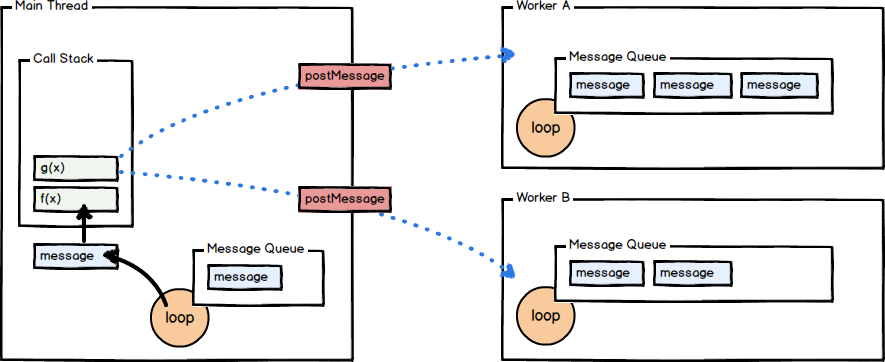
\includegraphics[width=0.8\textwidth]{web-workers}~\cite{Swenson-Healey2013}
	\end{center}
	
	\begin{alertblock}{Memory}
		Each Web Worker uses a distinct runtime environment (e.g. V8), therefore, the memory of each web worker is distinct too.
	\end{alertblock}

\end{frame}

\begin{frame}[fragile]{\enquote{Simple} Web Worker Example}
	\begin{columns}[t]
		\begin{column}{0.56\textwidth}
			\begin{block}{main.js}
				\begin{javascriptcode}
const worker = new Worker("./worker.js");
worker.postMessage(40);

worker.addEventListener(
	"message", 
	result => console.log(result.data)
);
				\end{javascriptcode}
			\end{block}
		\end{column}
		\pause
		\begin{column}{0.44\textwidth}
			\begin{block}{worker.js}
				\begin{javascriptcode}
function fib(num) {
	if(num <= 2) {
		return 1;
	}
	return fib(num - 1) + fib(num - 2);
}

onmessage = function (event) {
	const num = event.data;
	const result = fib(num);
	postMessage({ 
		number: num, 
		fib: result 
	});
};	
				\end{javascriptcode}
			\end{block}
		\end{column}

	\end{columns}

\end{frame}

\begin{frame}{But I also have to\dots}
	\begin{itemize}
		\item Handle Errors 
		\item Return a Promise in the UI-Thread
		\item Perform the Computation for multiple Items
		\item Besides, it should run on Node.JS too
	\end{itemize}
\end{frame}

\begin{frame}{And I don't like that\dots}
	\begin{itemize}
		\item code splitting is enforced by technology instead of by semantics
		\item the messaging model results in a clear seam 
		\item integration adds non inherent complexity
		\item the build gets far more complicated
	\end{itemize}
\end{frame}